\chapter[Analisi Rischi]{Analisi Rischi}
I flussi di cassa calcolati in precedenza sono puramente teorici, in quanto nella realtà essi sono influenzati, in maniera rilevante, da fattori esterni che possono determinare anche il fallimento di un progetto di investimento se non opportunamente stimati.
Nell'ambito di un call center i possibili rischi possono riguardare:
\begin{itemize}
\item il \textbf{guasto} delle varie apparecchiature. Si deve tener conto, infatti di un opportuno \textit{tasso di guasto} dovuto al ciclo di vita delle macchine che per quanto possa essere lungo è in ogni caso finito. In questa categoria, rientrano anche a quelli legati ad una non ottimale alimentazione elettrica. Si deve tenere presente, ad esempio, come il \textit{valore nominale} della fornitura di energia elettrica non assume lo stesso valore (in Italia 220 V AC), ma si ha una tolleranza del 10 \%. Inoltre, vi possono essere guasti sulla rete di distribuzione che possono determinare dei black-out anche di diverse ore;
\item le \textbf{malattie} dei centralinisti. I centralinisti, possono contrarre malanni che determinano un minor numero di chiamate possibili verso potenziali clienti e quindi determinano dei mancati guadagni rispetto alle stime ottimistiche;
\item la \textbf{variazione del tasso di cambio \euro -ALL}. Operando in un paese extracomunitario che, quindi, non adotta l'\euro ,siamo soggetti alle fluttuazioni del tasso di cambio nel mercato finanziario. Queste fluttuazioni possono determinare anche delle future corpose correzioni nell'investimento di nuovo capitale, in quanto un eccessivo rafforzamento dell'\textbf{ALL} rispetto all'\euro può comportare delle spese aggiuntive per garantire i servizi che sono stati prefissati.  
\end{itemize} 
La nostra analisi si è concentrata maggiormente nello studio del rischio delle \textbf{malattie} dei dipendenti e del \textbf{tasso di cambio}, in quanto abbiamo ritenuti trascurabili quelli legati ai \textbf{guasti}. Sistelia, infatti, garantisce una sostituzione delle apparecchiature nell'arco di 24 ore e per contrastare i guasti dovuti a malfunzionamenti nella rete di distribuzioneelettrica, ci fornisce un \textbf{gruppo di continuità \ac{UPS} Server}.

\section[Malattia Dipendenti]{Malattia Dipendenti}
	 \begin{tabular}{SS[table-format=2]}
 \toprule
 	{Anno} & {Giorni Malattia} \\
 \midrule
 	1990 & 10,7 \\
 	1991 & 11,1 \\
 	1992 & 11,1 \\
 	1993 & 11,4 \\
 	1994 & 11,4 \\
 	1995 & 11,6 \\
	1996 & 11,5 \\ 
	1997 & 11,3 \\
	1998 & 11,2 \\
	1999 & 11,5 \\
	2000 & 11,6 \\
	2001 & 11,8 \\
	2002 & 12,1 \\
	2003 & 12,2 \\
	2004 & 11,8 \\
	2006 & 11,4 \\
	2007 & 11,4 \\
	2008 & 11,6 \\
	2009 & 11,7 \\
	2010 & 11,6 \\
	2011 & 11,6 \\
	2012 & 11,7 \\							  
	2013 & 11,8 \\
	2014 & 11,8 \\

 \bottomrule
 \end{tabular} 

Prendendo in esame il campione caratterizzato dai valori precedentemente esposti, si possono calcolare le seguenti statistiche di interesse:

\begin{savenotes}
\begin{table}[htb]
\centering
 \caption{Statistiche}
 \begin{tabular}{p{5cm}D{,}{,}{5.5}}
 \toprule
 	\multicolumn{1}{c}{\textbf{Statistica}} & \multicolumn{1}{c}{\textbf{Valore}} \\
 \midrule 		
	\makebox[5cm][r]{Media Campionaria} & 12,03913\\
 	\makebox[5cm][r]{Varianza Campionaria Corretta} & 0,38525\\
 	\makebox[5cm][r]{Deviazione Standard Corretta} & 0,62068\\	
 \bottomrule
 \end{tabular} 
\end{table}
\end{savenotes} 
 
Da questi valori si può determinare il seguente intervallo di confidenza con il 95 \% di attendibilità

\[	\left [ 11,4184 ; 12,6598 \right]		\] 
 
 
consideriamo le seguenti ipotesi per ogni singolo centralinista: 
\begin{savenotes}
\begin{table}[htb]
\centering
 \caption{Assunzioni iniziali in un singolo mese}
 \begin{tabular}{p{7cm}D{,}{,}{5.2}}
 \toprule
 	& \multicolumn{1}{c}{\textbf{Quantita'}} \\
 \midrule 	
	\makebox[7cm][r]{Giorni lavorativi in un mese} & 18,50\\
	\makebox[7cm][r]{Giorni lavorativi in un anno} & 222,00\\
	\makebox[7cm][r]{Giorni assenza} & 12,00\\	
 	\makebox[7cm][r]{Probabilita' di stipulare un contratto (\%)\footnote{dati istat}} & 15,60\\
 \bottomrule
 \end{tabular} 
\end{table}
\end{savenotes}
%
%	Numero chiamate centralinisti
%
\begin{savenotes}
\begin{table}[htb]
\centering
 \caption{Numero contratti 29 centralinisti}
 \begin{tabular}{p{5cm}D{,}{,}{5.2}}
 \toprule
 	& \multicolumn{1}{c}{\textbf{Quantità}} \\
 \midrule 		
	\makebox[5cm][r]{Numero chiamate annuali} & 605172,00\\
 	\makebox[5cm][r]{Numero contratti annuali} & 94406,83 \\
 	\makebox[5cm][r]{Numero contratti mensili} & 7867,24\\  	
 \bottomrule
 \end{tabular} 
\end{table}
\end{savenotes}

\begin{comment}

\begin{savenotes}
\begin{table}[htb]
\centering
 \caption{Numero contratti centralinisti}
 \begin{tabular}{p{7cm}D{,}{,}{5.2}D{,}{,}{5.2}}
 \toprule
 	& \multicolumn{1}{c}{\textbf{Singolo Centralinista}} & \multicolumn{1}{c}{\textbf{29 Centralinisti}} \\
 \midrule 		
	\makebox[7cm][r]{Numero chiamate giornaliere} & 94,00 & 2820\\
 	\makebox[7cm][r]{Numero chiamate mensili} & 1739,00\footnote{(94,00*18,50)} & 52170\\
 	\makebox[7cm][r]{Contratti stipulati mensilmente} & 271,29 & 8138,52\\ 	
 	\makebox[7cm][r]{Chiamate mensili in caso di assenza per 12 giorni} & 611,00\footnote{(94,00*(18,50-12,00))} & 18330\\
 	\makebox[7cm][r]{Contratti stipulati in caso di assenza per 12 giorni} & 95,32\footnote{(611*0,156)} & 2859,48\\ 	
 \bottomrule
 \end{tabular} 
\end{table}
\end{savenotes}

\end{comment}
 
\begin{savenotes}
\begin{table}[htb]
\centering
 \caption{Variazione Fatturato}
 \begin{tabular}{p{8cm}D{,}{,}{5.2}D{,}{,}{5.2}}
 \toprule
 	& \multicolumn{1}{c}{\textbf{VAN PAREGGIO}} & \multicolumn{1}{c}{\textbf{VAN CASO REALE}} \\
 \midrule
 	\makebox[8cm][r]{Probabilita' di successo di un contratto (\%)} & 11,54 & 15,00\\
 \midrule
	\makebox[8cm][r]{Numero contratti stipulati (1 mese)} & 8138,52 & 8138,52\\
	\makebox[8cm][r]{Numero contratti stipulati (30 malati in 1 mese)} & 2859,48 & 2859,48\\
 \midrule	
	\makebox[8cm][r]{Numero contratti successo (1 mese)} & 939,50 & 1220,78\\
	\makebox[8cm][r]{Numero contratti successo (30 malati in 1 mese)} & 329,98 & 428,92\\
 \midrule	
	\makebox[8cm][r]{Fatturato Lordo (\euro) (1 mese)} & 75160,00 & 97662,40\\
	\makebox[8cm][r]{Fatturato Lordo (\euro) (30 malati in 1 mese)} & 26398,72 & 34313,76\\	
 \midrule	
	\makebox[8cm][r]{Fatturato Netto (\euro) (1 mese)} & 65314,04 & 84917,46\\
	\makebox[8cm][r]{Fatturato Netto (\euro) (30 malati in 1 mese)} & 22953,69 & 29835,81\\	
 \bottomrule
 \end{tabular} 
\end{table}\
\end{savenotes}

\section[Variazione Tasso Cambio]{Variazione Tasso Cambio}
	L'impatto della variazione del tasso di cambio sull'analisi dei flussi mensili è stato valutato, considerando il tasso medio giornaliero, esaminando un campione dei tassi dal 07/07/2016 al 02/01/2017 (nell'analisi proposta è stato preso come riferimento il tasso di cambio del 15/12/2016 pari a $ \mbox{\ 1\: \euro \: = 136,51 ALL} $ evidenziato in \textbf{\textcolor{gray}{grigio}} nella tabella seguente).
\newline
\begin{longtable}{p{3cm}D{,}{,}{5.2}}
% didascalia ed etichetta
\caption{Andamento Tasso di Cambio (\euro -LEK)}\\
% intestazione iniziale
\toprule
	\makebox[3cm][c]{\textbf{Data}} & \multicolumn{1}{c}{\textbf{LEK}} \\
\midrule
\label{cambio_euro_lek}
\endfirsthead
% intestazione normale
\multicolumn{2}{l}{\footnotesize\itshape\tablename~\thetable:
continua dalla pagina precedente} \\
\toprule
	\makebox[3cm][c]{\textbf{Data}} & \multicolumn{1}{c}{\textbf{LEK}} \\
\midrule
\endhead
% piede normale
\midrule
\multicolumn{2}{r}{\footnotesize\itshape\tablename~\thetable:
continua nella prossima pagina} \\
\endfoot
% piede finale
\bottomrule
\multicolumn{2}{r}{\footnotesize\itshape\tablename~\thetable:
si conclude dalla pagina precedente} \\
\endlastfoot
% corpo della tabella
	\makebox[3cm][c]{$07/07/2016$} & 136,78\\
	\makebox[3cm][c]{$08/07/2016$} & 136,54\\	
 	\makebox[3cm][c]{$10/07/2016$} & 136,55\\
	\makebox[3cm][c]{$11/07/2016$} & 136,68\\
	\makebox[3cm][c]{$12/07/2016$} & 136,73\\	
 	\makebox[3cm][c]{$13/07/2016$} & 136,83\\
 	\makebox[3cm][c]{$14/07/2016$} & 136,77\\
	\makebox[3cm][c]{$15/07/2016$} & 136,52\\	
 	\makebox[3cm][c]{$17/07/2016$} & 136,53\\
	\makebox[3cm][c]{$18/07/2016$} & 136,57\\	
 	\makebox[3cm][c]{$19/07/2016$} & 136,43\\
 	\makebox[3cm][c]{$20/07/2016$} & 136,40\\
	\makebox[3cm][c]{$21/07/2016$} & 135,95\\	
 	\makebox[3cm][c]{$22/07/2016$} & 135,18\\
 	\makebox[3cm][c]{$24/07/2016$} & 135,17\\
	\makebox[3cm][c]{$25/07/2016$} & 135,98\\	
 	\makebox[3cm][c]{$26/07/2016$} & 136,34\\
 	\makebox[3cm][c]{$27/07/2016$} & 137,15\\
	\makebox[3cm][c]{$28/07/2016$} & 136,18\\	
 	\makebox[3cm][c]{$29/07/2016$} & 138,62\\
  	\makebox[3cm][c]{$31/07/2016$} & 136,12\\
	\makebox[3cm][c]{$01/08/2016$} & 136,11\\	
 	\makebox[3cm][c]{$02/08/2016$} & 136,80\\	
	\makebox[3cm][c]{$03/08/2016$} & 138,34\\	
	\makebox[3cm][c]{$04/08/2016$} & 136,06\\	
	\makebox[3cm][c]{$05/08/2016$} & 135,52\\	
	\makebox[3cm][c]{$07/08/2016$} & 135,55\\	
	\makebox[3cm][c]{$08/08/2016$} & 135,48\\	
	\makebox[3cm][c]{$09/08/2016$} & 136,21\\	
	\makebox[3cm][c]{$10/08/2016$} & 135,95\\	
	\makebox[3cm][c]{$11/08/2016$} & 136,01\\	
	\makebox[3cm][c]{$12/08/2016$} & 136,17\\	
	\makebox[3cm][c]{$14/08/2016$} & 136,13\\	
	\makebox[3cm][c]{$15/08/2016$} & 136,33\\	
	\makebox[3cm][c]{$16/08/2016$} & 135,77\\	
	\makebox[3cm][c]{$17/08/2016$} & 136,30\\	
	\makebox[3cm][c]{$18/08/2016$} & 137,37\\	
	\makebox[3cm][c]{$19/08/2016$} & 137,26\\	
	\makebox[3cm][c]{$21/08/2016$} & 136,62\\	
	\makebox[3cm][c]{$22/08/2016$} & 136,63\\	
	\makebox[3cm][c]{$23/08/2016$} & 136,86\\	
	\makebox[3cm][c]{$24/08/2016$} & 136,43\\	
	\makebox[3cm][c]{$25/08/2016$} & 137,22\\	
	\makebox[3cm][c]{$26/08/2016$} & 135,97\\	
	\makebox[3cm][c]{$28/08/2016$} & 135,77\\	
	\makebox[3cm][c]{$29/08/2016$} & 137,18\\	
	\makebox[3cm][c]{$30/08/2016$} & 136,64\\	
	\makebox[3cm][c]{$31/08/2016$} & 137,69\\
	\makebox[3cm][c]{$01/09/2016$} & 137,54\\
	\makebox[3cm][c]{$02/09/2016$} & 137,06\\
	\makebox[3cm][c]{$04/09/2016$} & 137,05\\
	\makebox[3cm][c]{$05/09/2016$} & 137,35\\
	\makebox[3cm][c]{$06/09/2016$} & 138,64\\
	\makebox[3cm][c]{$07/09/2016$} & 137,62\\
	\makebox[3cm][c]{$08/09/2016$} & 137,28\\
	\makebox[3cm][c]{$09/09/2016$} & 137,16\\
	\makebox[3cm][c]{$11/09/2016$} & 137,17\\
	\makebox[3cm][c]{$12/09/2016$} & 137,37\\
	\makebox[3cm][c]{$13/09/2016$} & 137,63\\
	\makebox[3cm][c]{$14/09/2016$} & 138,04\\
	\makebox[3cm][c]{$15/09/2016$} & 137,34\\
	\makebox[3cm][c]{$16/09/2016$} & 136,21\\
	\makebox[3cm][c]{$18/09/2016$} & 136,21\\
	\makebox[3cm][c]{$19/09/2016$} & 137,14\\
	\makebox[3cm][c]{$20/09/2016$} & 137,17\\
	\makebox[3cm][c]{$21/09/2016$} & 137,67\\
	\makebox[3cm][c]{$22/09/2016$} & 137,84\\
	\makebox[3cm][c]{$23/09/2016$} & 137,04\\
	\makebox[3cm][c]{$25/09/2016$} & 137,05\\
	\makebox[3cm][c]{$26/09/2016$} & 137,42\\
	\makebox[3cm][c]{$27/09/2016$} & 137,19\\
	\makebox[3cm][c]{$28/09/2016$} & 137,01\\
	\makebox[3cm][c]{$29/09/2016$} & 137,47\\
	\makebox[3cm][c]{$30/09/2016$} & 137,48\\
	\makebox[3cm][c]{$02/10/2016$} & 137,26\\
	\makebox[3cm][c]{$03/10/2016$} & 136,93\\
	\makebox[3cm][c]{$04/10/2016$} & 137,40\\
	\makebox[3cm][c]{$05/10/2016$} & 137,24\\
	\makebox[3cm][c]{$06/10/2016$} & 136,90\\
	\makebox[3cm][c]{$07/10/2016$} & 138,20\\
	\makebox[3cm][c]{$09/10/2016$} & 137,95\\
	\makebox[3cm][c]{$10/10/2016$} & 137,07\\
	\makebox[3cm][c]{$11/10/2016$} & 136,03\\
	\makebox[3cm][c]{$12/10/2016$} & 136,92\\
	\makebox[3cm][c]{$13/10/2016$} & 137,00\\
	\makebox[3cm][c]{$14/10/2016$} & 136,05\\
	\makebox[3cm][c]{$16/10/2016$} & 136,03\\
	\makebox[3cm][c]{$17/10/2016$} & 137,32\\
	\makebox[3cm][c]{$18/10/2016$} & 137,09\\
	\makebox[3cm][c]{$19/10/2016$} & 137,04\\
	\makebox[3cm][c]{$20/10/2016$} & 135,88\\
	\makebox[3cm][c]{$21/10/2016$} & 135,53\\
	\makebox[3cm][c]{$23/10/2016$} & 136,07\\
	\makebox[3cm][c]{$24/10/2016$} & 136,03\\
	\makebox[3cm][c]{$25/10/2016$} & 136,23\\
	\makebox[3cm][c]{$26/10/2016$} & 136,57\\
	\makebox[3cm][c]{$27/10/2016$} & 136,42\\
	\makebox[3cm][c]{$28/10/2016$} & 137,42\\
	\makebox[3cm][c]{$30/10/2016$} & 136,54\\
	\makebox[3cm][c]{$31/10/2016$} & 137,04\\	
	\makebox[3cm][c]{$01/11/2016$} & 137,48\\
	\makebox[3cm][c]{$02/11/2016$} & 137,06\\
	\makebox[3cm][c]{$03/11/2016$} & 136,47\\
	\makebox[3cm][c]{$04/11/2016$} & 137,19\\
	\makebox[3cm][c]{$06/11/2016$} & 136,41\\
	\makebox[3cm][c]{$07/11/2016$} & 136,66\\
	\makebox[3cm][c]{$08/11/2016$} & 136,57\\
	\makebox[3cm][c]{$09/11/2016$} & 134,87\\
	\makebox[3cm][c]{$10/11/2016$} & 136,32\\
	\makebox[3cm][c]{$11/11/2016$} & 135,98\\
	\makebox[3cm][c]{$13/11/2016$} & 136,00\\
	\makebox[3cm][c]{$14/11/2016$} & 136,00\\
	\makebox[3cm][c]{$15/11/2016$} & 135,89\\
	\makebox[3cm][c]{$16/11/2016$} & 136,05\\
	\makebox[3cm][c]{$17/11/2016$} & 134,59\\
	\makebox[3cm][c]{$18/11/2016$} & 135,38\\
	\makebox[3cm][c]{$20/11/2016$} & 135,38\\
	\makebox[3cm][c]{$21/11/2016$} & 135,80\\
	\makebox[3cm][c]{$22/11/2016$} & 135,80\\
	\makebox[3cm][c]{$23/11/2016$} & 135,94\\
	\makebox[3cm][c]{$24/11/2016$} & 135,81\\
	\makebox[3cm][c]{$25/11/2016$} & 136,11\\
	\makebox[3cm][c]{$27/11/2016$} & 136,19\\
	\makebox[3cm][c]{$28/11/2016$} & 135,73\\
	\makebox[3cm][c]{$29/11/2016$} & 136,37\\
	\makebox[3cm][c]{$30/11/2016$} & 135,68\\
	\makebox[3cm][c]{$01/12/2016$} & 135,77\\
	\makebox[3cm][c]{$02/12/2016$} & 136,05\\
	\makebox[3cm][c]{$04/12/2016$} & 134,45\\
	\makebox[3cm][c]{$05/12/2016$} & 136,84\\
	\makebox[3cm][c]{$06/12/2016$} & 137,10\\
	\makebox[3cm][c]{$07/12/2016$} & 135,81\\
	\makebox[3cm][c]{$08/12/2016$} & 135,78\\
	\makebox[3cm][c]{$09/12/2016$} & 135,86\\
	\makebox[3cm][c]{$11/12/2016$} & 135,65\\
	\makebox[3cm][c]{$12/12/2016$} & 135,81\\
	\makebox[3cm][c]{$13/12/2016$} & 135,63\\
	\makebox[3cm][c]{$14/12/2016$} & 134,65\\
	\rowcolor[gray]{.7}\makebox[3cm][c]{$15/12/2016$} & 136,51\\
	\makebox[3cm][c]{$16/12/2016$} & 135,73\\
	\makebox[3cm][c]{$18/12/2016$} & 135,66\\
	\makebox[3cm][c]{$19/12/2016$} & 135,17\\
	\makebox[3cm][c]{$20/12/2016$} & 134,45\\
	\makebox[3cm][c]{$21/12/2016$} & 134,37\\
	\makebox[3cm][c]{$22/12/2016$} & 134,43\\
	\makebox[3cm][c]{$23/12/2016$} & 134,35\\
	\makebox[3cm][c]{$25/12/2016$} & 134,60\\	
	\makebox[3cm][c]{$26/12/2016$} & 134,38\\
	\makebox[3cm][c]{$27/12/2016$} & 134,52\\
	\makebox[3cm][c]{$28/12/2016$} & 134,94\\
	\makebox[3cm][c]{$29/12/2016$} & 134,86\\
	\makebox[3cm][c]{$30/12/2016$} & 134,90\\
	\makebox[3cm][c]{$01/01/2017$} & 134,95\\
	\makebox[3cm][c]{$02/01/2017$} & 134,39\\				
\end{longtable}
Le principali grandezze che lo caratterizzano sono pari a (per approfondimenti si rimanda all'appendice \ref{sec:stimatori_tasso_cambio}):

\begin{savenotes}
\begin{table}[htb]
\centering
 \caption{Grandezze}
 \label{table:grandezze_cambio}
 \begin{tabular}{p{5cm}D{,}{,}{5.5}}
 \toprule
 	\multicolumn{1}{c}{\textbf{Grandezza}} & \multicolumn{1}{c}{\textbf{Valore}} \\
 \midrule 		
	\makebox[5cm][r]{Media Campionaria} & 136,47083\\
 	\makebox[5cm][r]{Varianza Campionaria Corretta} & 0,88366\\
 	\makebox[5cm][r]{Deviazione Standard Corretta} & 0,94003\\	
 \bottomrule
 \end{tabular} 
\end{table}
\end{savenotes}
L'intervallo di confidenza, di livello $0,9$ ad esse associato è pari a:
\begin{equation}
	\label{eq:intervallo_confidenza_tasso_cambio}
	\begin{split}
		\left [ 135,53 ; 137,41 \right]	 
	\end{split}
\end{equation}

\subsection[Casi di Studio]{Casi di Studio}
Si è analizzato, nel dettaglio, l'impatto che può presentare una variazione del tasso di cambio nel caso realistico in cui i dipendenti si possano assentare per malattia, in maniera uniforme durante l'arco dell'anno lavorativo (non si sono considerati i casi limite, ovvero la situazione per cui gli assenti per malattia si concentrano nei mesi di Gennaio e Dicembre). \newline Si è studiato, in particolare, il caso in cui il \emph{lek} possa subire, rispetto all'\emph{euro}:
\begin{itemize}
\item un \textbf{rafforzamento}, quindi si dovranno spendere \underline{più} \textit{euro} per acquistare la stessa quantità di \textit{lek} (\textbf{CASO PEGGIORE});
\item un \textbf{deprezzamento}, viceversa si dovranno utilizzare \underline{meno} \textit{euro} per acquistare la stessa quantità di \textit{lek} (\textbf{CASO MIGLIORE});
\end{itemize} 
Per tener conto di questo fenomeno si introduce l'elemento adimensionale $ f $ ($fattore \thinspace di \thinspace aggiustamento$) definito come il rapporto tra un tasso di cambio \emph{euro-lek} di riferimento fisso $x$ ed uno variabile $y$:
\begin{equation}
\label{eq:fattore_aggiustamento}
\begin{split}
	f = \frac{x}{y}
\end{split}
\end{equation}
questo fattore terrà conto, di conseguenza delle variazioni del tasso di cambio rispetto ad uno ben definito.
Nell'analisi proposta il valore di riferimento $x$, è quello del tasso di cambio al 15/12/2016:
\begin{equation}
\label{eq:fattore_aggiustamento_rif}
\begin{split}
	x = 136,51
\end{split}
\end{equation}
A titolo di esempio si consideri la seguente sezione della tabella (\ref{cambio_euro_lek}):
\begin{savenotes}
\begin{table}[htb]
\centering
 \caption{Tasso di Cambio (\euro -LEK)}
 \begin{tabular}{p{5cm}D{,}{,}{5.5}}
 \toprule
 	\multicolumn{1}{c}{\textbf{Giorno}} & \multicolumn{1}{c}{\textbf{Valore Cambio}} \\
 \midrule 		
	\makebox[3cm][c]{$06/12/2016$} & 137,10\\
	\makebox[3cm][c]{$07/12/2016$} & 135,81\\
	\makebox[3cm][c]{$08/12/2016$} & 135,78\\
	\makebox[3cm][c]{$09/12/2016$} & 135,86\\
	\makebox[3cm][c]{$11/12/2016$} & 135,65\\
	\makebox[3cm][c]{$12/12/2016$} & 135,81\\
	\makebox[3cm][c]{$13/12/2016$} & 135,63\\
	\makebox[3cm][c]{$14/12/2016$} & 134,65\\
	\rowcolor[gray]{.7}\makebox[3cm][c]{$15/12/2016$} & 136,51\\
	\makebox[3cm][c]{$16/12/2016$} & 135,73\\
	\makebox[3cm][c]{$18/12/2016$} & 135,66\\
	\makebox[3cm][c]{$19/12/2016$} & 135,17\\
	\makebox[3cm][c]{$20/12/2016$} & 134,45\\
	\makebox[3cm][c]{$21/12/2016$} & 134,37\\
 \bottomrule
 \end{tabular} 
\end{table}
\end{savenotes}
Il \emph{fattore di aggiustamento} calcolato con il tasso del $06/12/2016$ è pari a:
\begin{equation}
\label{eq:example_1_fattore_aggiustamento}
\begin{split}
	f = \frac{tasso \thinspace cambio \thinspace 15/12/2016}{tasso \thinspace cambio \thinspace 06/12/2016} = \frac{136,51}{137,10} = 0,9956
\end{split}
\end{equation}

calcolando il prodotto tra (\ref{eq:example_1_fattore_aggiustamento}) ed una certa quantità di \emph{euro}, ad esempio $ z = \mbox{\euro \thinspace 100}$:

\begin{eqnarray}
\label{eq:euro_example1}
	\gamma _1 (\mbox{\euro})& = & 0,9956 \cdot z 	\nonumber \\
			  & = & 0,9956 \cdot 100,00 \thinspace \mbox{\euro} \nonumber \\
			  & = & 99,56 \thinspace \mbox{\euro}
\end{eqnarray}
si ottiene il valore di $z = \mbox{\euro \thinspace 100}$ con un cambio \underline{sfavorevole} rispetto a quello di riferimento (ovvero quello del $06/12/2016$). A parità di prezzo in lek, quindi, dovremmo spendere più \textit{euro} per acquistare un certo bene.\newline
Analogamente, ripetendo i calcoli precedenti con il tasso del $02/01/2017$:
\begin{equation}
\label{eq:example_2_fattore_aggiustamento}
\begin{split}
	f = \frac{tasso \thinspace cambio \thinspace 15/12/2016}{tasso \thinspace cambio \thinspace 20/01/2016} = \frac{136,51}{134,45} = 1,015
\end{split}
\end{equation}
\begin{eqnarray}
\label{eq:euro_example2}
	\gamma _2 (\mbox{\euro})& = & 1,015 \cdot z 	\nonumber \\
			  & = & 1,015 \cdot 100,00 \thinspace \mbox{\euro} \nonumber \\
			  & = & 101,50 \thinspace \mbox{\euro}
\end{eqnarray}
La formula del calcolo del VAN dovrà tener conto di queste variazioni, pertanto la (\ref{eq:van_caso_studio_2}) assumerà la seguente forma:
	\begin{eqnarray}
	\label{eq:van_caso_studio_tassocambio}
 		y(x) & = & - 56\thinspace 170,20 + \sum_{k=1}^{12} \frac{x - 60\thinspace 131,27 \cdot f}{(1+0,058)^k} \nonumber \\
 		 & = & -56\thinspace 170,20 + (x - 60\thinspace 131,27 \cdot f) \cdot \underbrace{\sum_{k=1}^{12} \frac{1} {(1+0,058)^{k}}}_{{}=8,47654} \nonumber \\
 		 & = & -56\thinspace 170,20 + (x - 60\thinspace 131,27 \cdot f) \cdot 8,47654		
	\end{eqnarray}  		

	\begin{tcolorbox}[colframe=blue!75!black,adjusted title=\textbf{Osservazione!}]
		Nella formula (\ref{eq:van_caso_studio_tassocambio}) si è considerato la variazione del tasso \emph{euro}-\emph{lek} soltanto per gli \emph{\ac{OPEX}}. \newline Rispetto a (\ref{eq:van_caso_studio_2}) il \emph{peso} quest'ultimi sono modificati in:
		\[ 60\thinspace 131,27 \cdot f \] 
	In linea teorica anche i \emph{\ac{CAPEX}} e le entrate mensile nette \emph{x} dovranno tener conto di questo fattore. Nel caso analizzato, ciò non si verifica, perchè, per quanto riguarda le entrate \emph{x}, Sistelia retribuisce direttamente in \emph{euro}, pertanto questa quantità non è influita dal cambio.\newline Un discorso analogo riguarda i \emph{\ac{CAPEX}}, in quanto i prezzi delle attrezzature sono fornite da Sistelia e sono forniti anch'essi in \emph{euro}.
	\end{tcolorbox} 
\subsubsection[Caso Peggiore - Deprezzamento dell'euro]{Caso Peggiore - Deprezzamento dell'euro}
\label{sec:cambio_favorevole}
La situazione migliore si presenta, quando l'\emph{euro} vale $135,53 \thinspace lek$, ovvero quando il tasso \emph{euro-lek} presenta un valore pari al limite sinistro dell'intervallo di confidenza (\ref{eq:intervallo_confidenza_tasso_cambio}). Il tasso di cambio risulterebbe sfavorevole rispetto al caso medio (ovvero alla \textit{media campionaria} (\ref{table:grandezze_cambio})) in cui, invece, l'euro è scambiato con $136,47 \thinspace lek$.\newline
In queste condizioni il valore del \textit{fattore di aggiustamento}  (\ref{eq:fattore_aggiustamento}) è uguale a:
\begin{equation}
\label{eq:fattore_aggiustamento_caso_migliore}
\begin{split}
f = \frac{136,47}{135,35} = 1,007
\end{split}
\end{equation}
quindi la formula del \emph{\ac{VAN}} (\ref{eq:van_caso_studio_tassocambio}) diventa:

\begin{eqnarray}
\label{eq:van_caso_migliore}
 		y(x) & = & -56\thinspace 170,20 + (x - 60\thinspace 131,27 \cdot f) \cdot 8,47654 \nonumber \\
 			 & = & -56\thinspace 170,20 + (x - 60\thinspace 131,27 \cdot 1,007) \cdot 8,47654 \nonumber \\
 			 & = & -569\thinspace 443,25 + x \cdot 8,47654
\end{eqnarray}

Il valore di (\ref{eq:van_caso_migliore}) in corrispondenza del flusso di cassa mensile $ x = \mbox{73\thinspace 925,12 \euro}$ (\ref{table:van_malati_uniforme_anno}):
\begin{eqnarray}
\label{eq:van_flusso_cassa_malati_uniforme_caso_migliore}
 		y(x) & = & -569\thinspace 443,25 + x \cdot 8,47654 \nonumber \\
 			 & = & -569\thinspace 443,25 + 73\thinspace 925,12 \cdot 8,47654 \nonumber \\
 			 & = & 57\thinspace 185,985 \simeq 57\thinspace 185,99
\end{eqnarray}

\subsubsection[Caso Migliore - Rafforzamento dell'euro]{Caso Migliore - Rafforzamento dell'euro}
\label{sec:cambio_sfavorevole}
La situazione peggiore si presenta, invece, quando l'\emph{euro} vale $137,41 \thinspace lek$, ovvero quando il tasso \emph{euro-lek} presenta un valore pari al limite destro dell'intervallo di confidenza (\ref{eq:intervallo_confidenza_tasso_cambio}). Il tasso di cambio risulterebbe sfavorevole rispetto al caso medio (ovvero alla \textit{media campionaria} (\ref{table:grandezze_cambio})) in cui, invece, l'euro è scambiato con $136,47 \thinspace lek$.\newline
In queste condizioni il valore del \textit{fattore di aggiustamento}  (\ref{eq:fattore_aggiustamento}) è uguale a:
\begin{equation}
\label{eq:fattore_aggiustamento_caso_peggiore}
\begin{split}
f = \frac{136,47}{137,41} = 0,993
\end{split}
\end{equation}
quindi la formula del \emph{\ac{VAN}} (\ref{eq:van_caso_studio_tassocambio}) diventa:

\begin{eqnarray}
\label{eq:van_caso_peggiore}
 		y(x) & = & -56\thinspace 170,20 + (x - 60\thinspace 131,27 \cdot f) \cdot 8,47654 \nonumber \\
 			 & = & -56\thinspace 170,20 + (x - 60\thinspace 131,27 \cdot 0,993) \cdot 8,47654 \nonumber \\
 			 & = & -562\thinspace 307,38 + x \cdot 8,47654
\end{eqnarray}

Il valore di (\ref{eq:van_caso_peggiore}) in corrispondenza del flusso di cassa mensile $ x = \mbox{73\thinspace 925,12 \euro}$ (\ref{table:van_malati_uniforme_anno}):
\begin{eqnarray}
\label{eq:van_flusso_cassa_malati_uniforme_caso_peggiore}
 		y(x) & = & -562\thinspace 307,38 + x \cdot 8,47654 \nonumber \\
 			 & = & -562\thinspace 307,38 + 73\thinspace 925,12 \cdot 8,47654 \nonumber \\
 			 & = & 64\thinspace 321,8567 \simeq 64\thinspace 321,86
\end{eqnarray}


\section[Sintesi Risultati]{Sintesi Risultati}
I risultati ottenuti in (\ref{sec:cambio_favorevole}) e in (\ref{sec:cambio_sfavorevole}) possono essere riassunti nella seguente tabella:

\begin{savenotes}
\begin{table}[htb]
\centering
 \caption{Variazione VAN (Caso di studio 15 \% comprensivo del rischio malattie)}
 \begin{tabular}{D{,}{,}{5.2}D{,}{,}{4.3}D{,}{,}{7.2}}
 \toprule
 	\multicolumn{1}{c}{\textbf{Cambio \emph{euro-lek}}} & 
 	\multicolumn{1}{c}{\textbf{Aggiustamento}}			&
 	\multicolumn{1}{c}{\textbf{Valore VAN (\euro)}} \\
 \midrule 		
	135,53 & 1,007 & 57\thinspace 185,99 \\
	137,41 & 0,993 & 64\thinspace 321,86 \\	
 \bottomrule
 \end{tabular} 
\end{table}
\end{savenotes}
	
\section[Diagramma Tornado]{Diagramma Tornado}	
	I risultati ottenuti dall'analisi dei rischi possono essere riassunti efficacemente in una diagramma definito che permette di visualizzare efficacemente la valutazione della variazione del VAN in funzione di un rischio considerato singolarmente.
\begin{figure}[htbp]
\centering
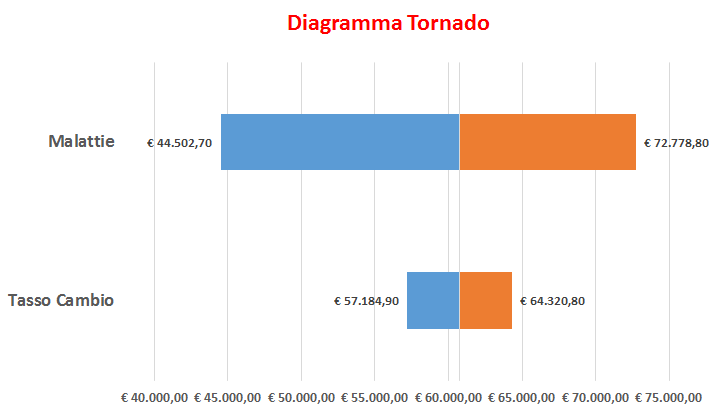
\includegraphics[scale=0.7]{immagini/Tornado.png}
\caption{Diagramma Tornado per i rischi Malattie e Tasso di Cambio \label{fig:tornado}}
\end{figure}